\documentclass[journal,12pt,twocolumn]{IEEEtran}
\usepackage{cite}
\usepackage{amsmath,amssymb,amsfonts,amsthm}
\usepackage{algorithmic}
\usepackage{graphicx}
\usepackage{textcomp}
\usepackage{xcolor}
\usepackage{txfonts}
\usepackage{listings}
\usepackage{enumitem}
\usepackage{mathtools}
\usepackage{gensymb}
\usepackage{comment}
\usepackage[breaklinks=true]{hyperref}
\usepackage{tkz-euclide}
\usepackage{listings}
\usepackage{gvv}
\usepackage{braket}
\def\inputGnumericTable{}
\usepackage[latin1]{inputenc}
\usepackage{color}
\usepackage{array}
\usepackage{longtable}
\usepackage{calc}
\usepackage{multirow}
\usepackage{hhline}
\usepackage{ifthen}
\usepackage{lscape}

\newtheorem{theorem}{Theorem}[section]
\newtheorem{problem}{Problem}
\newtheorem{proposition}{Proposition}[section]
\newtheorem{lemma}{Lemma}[section]
\newtheorem{corollary}[theorem]{Corollary}
\newtheorem{example}{Example}[section]
\newtheorem{definition}[problem]{Definition}
\newcommand{\BEQA}{\begin{eqnarray}}
\newcommand{\EEQA}{\end{eqnarray}}
\newcommand{\define}{\stackrel{\triangle}{=}}
\theoremstyle{remark}
\newtheorem{rem}{Remark}
\begin{document}

\bibliographystyle{IEEEtran}
\vspace{3cm}

\title{GATE 2022 BM-42}
\author{EE23BTECH11201 - Abburi Tanusha$^{*}$% <-this % stops a space
}
\maketitle
\newpage
\bigskip

\renewcommand{\thefigure}{\theenumi}
\renewcommand{\thetable}{\theenumi}

\vspace{3cm}

\maketitle
\textbf{Question:} 
If \begin{align*}
 g(t) = \frac{df(t)}{dt} \\
 F(s) = \frac{1+s}{s^2+12s+32} 
 \end{align*} where $F(s)$ is the Laplace transform of the function $f(t)$, then what is the value of $g(t)$ at $t=0$ ?\\
\hfill(GATE 2022 BM)\\
\textbf{Solution:} 
\begin{table}[h!]
\centering
\resizebox{6cm}{!}{
\begin{table}[H]
    \centering
    \renewcommand\thetable{1}
    \setlength{\extrarowheight}{9pt}
    \resizebox{0.51\textwidth}{!}{
    \begin{tabular}{|c|c|c|}
    \hline
    \textbf{$r\brak{i}$} & \textbf{$p\brak{i}$} & \textbf{$k\brak{i}$} \\ \hline
    $0.06029142-0.14682007jj$ &0.88475217+0.0445749j&$2.19006287\times10^{-5}$  \\ \hline
    $0.06029142+0.14682007jj$ &0.88475217-0.0445749j&$-$  \\ \hline
    $-0.06029459+0.02518904j$ &0.94427798+0.11485352jj&$-$  \\ \hline
    $-0.06029459-0.02518904j$ & 0.94427798-0.11485352j&$-$  \\ \hline
    \end{tabular}}
    \caption{Values of $ r(i) , p(i) , k(i)$}
    \label{tab:values of r(i) , p(i) , k(i)}
    \end{table}

}
\caption{Given Parameters}
\label{tab:tanu_tabel}
\end{table}
\begin{align}
F(s) &= \frac{1+s}{(s+4)(s+8)}
\end{align}
Using partial fraction decomposition:
\begin{align}
F(s) &= \frac{A}{s+4} + \frac{B}{s+8} \\
1+s &= A(s+8) + B(s+4) \\
1+s &= (A+B)s + 8A + 4B
\end{align}
Comparing coefficients:
\begin{align}
A+B &= 1 \\
8A + 4B &= 1
\end{align}
By Solving these equations, we will get
 \begin{align}
  A &= -\frac{3}{4} \\
  B &= \frac{7}{4}  \\
F(s) &= \frac{\frac{7}{4}}{s+8} - \frac{\frac{3}{4}}{s+4} 
\end{align}
Inverse Laplace transform of $F(s)$ 
\begin{align}
f(t) &= \mathcal{L}^{-1}\left(\frac{\frac{7}{4}}{s+8}\right) - \mathcal{L}^{-1}\left(\frac{\frac{3}{4}}{s+4}\right) \\
&= \frac{7}{4}\mathcal{L}^{-1}\left(\frac{1}{s+8}\right) - \frac{3}{4}\mathcal{L}^{-1}\left(\frac{1}{s+4}\right) \\
&= \frac{7}{4}e^{-8t} - \frac{3}{4}e^{-4t}
\end{align}
\begin{align}
g(t) &= \frac{d}{dt}\left(\frac{7}{4}e^{-8t} - \frac{3}{4}e^{-4t}\right) \\
&= \frac{7}{4}\cdot(-8)e^{-8t} - \frac{3}{4}\cdot(-4)e^{-4t} \\
&= -14e^{-8t} + 3e^{-4t} \\
g(0) &= -14 \times 1 + 3 \times 1 \\
&= -14 + 3 = -11
\end{align}
The value of $g(t)$ at $t = 0$ is $-11$ \\
\begin{figure}[h!]
\centering
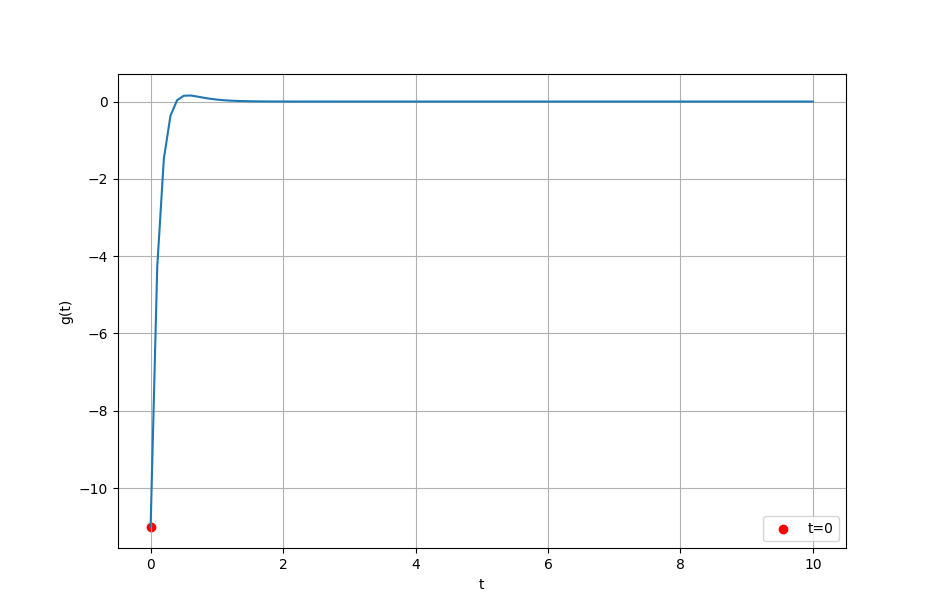
\includegraphics[width=\columnwidth]{figs/stem_plot.png}
\label{fig:tansh_plott}
\caption{plot g(t) vs t }
\end{figure}
\end{document}

